% This file was created with tikzplotlib v0.9.16.
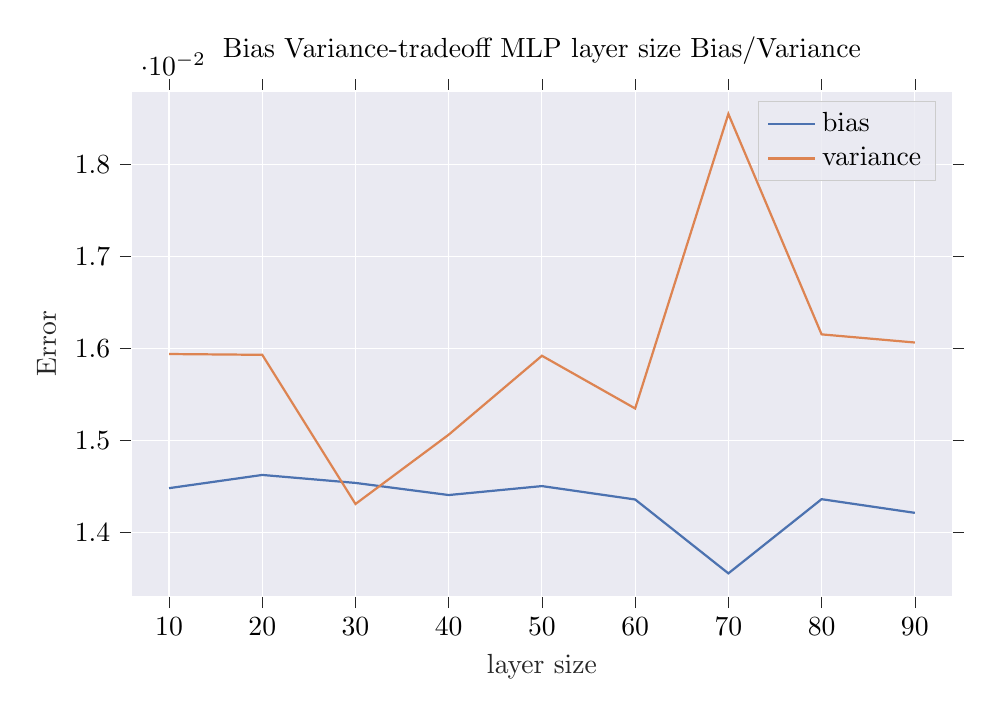
\begin{tikzpicture}

\definecolor{color0}{rgb}{0.917647058823529,0.917647058823529,0.949019607843137}
\definecolor{color1}{rgb}{0.298039215686275,0.447058823529412,0.690196078431373}
\definecolor{color2}{rgb}{0.866666666666667,0.517647058823529,0.32156862745098}

\begin{axis}[
width=12cm,height=8cm,axis background/.style={fill=color0},
axis line style={white},
legend cell align={left},
legend style={fill opacity=0.8, draw opacity=1, text opacity=1, draw=white!80!black, fill=color0},
tick align=outside,
title={Bias Variance-tradeoff MLP layer size Bias/Variance},
x grid style={white},
xlabel=\textcolor{white!15!black}{layer size},
xmajorgrids,
xmajorticks=true,
xmin=6, xmax=94,
xtick style={color=white!15!black},
y grid style={white},
ylabel=\textcolor{white!15!black}{Error},
ymajorgrids,
ymajorticks=true,
ymin=0.0133084491511077, ymax=0.0187989401113317,
ytick style={color=white!15!black}
]
\addplot [thick, color1]
table {%
10 0.0144836902618408
20 0.01462721824646
30 0.0145405530929565
40 0.0144089460372925
50 0.0145062208175659
60 0.0143606662750244
70 0.013558030128479
80 0.0143638849258423
90 0.0142154693603516
};
\addlegendentry{bias}
\addplot [thick, color2]
table {%
10 0.0159409046173096
20 0.0159322023391724
30 0.014311671257019
40 0.0150647163391113
50 0.015921950340271
60 0.0153495073318481
70 0.0185493230819702
80 0.016154408454895
90 0.0160659551620483
};
\addlegendentry{variance}
\end{axis}

\end{tikzpicture}
